% !TeX spellcheck = hu_HU
% !TeX encoding = UTF-8
\chapter{Alkalmazási példák}

\section{Párhuzamos fordítás}

A manapság egyre nagyobbra növő kódbázisok problémája, hogy egy-egy teljes fordítás nagyon sokáig tart.
Ahogy növekszik a forrásfájlok mérete és azok száma, a komplikált, nagy feladatokat megoldó projektek fordítása egyre több és több ideig tart.
Az egyik legjobb nyílt forráskódú projekt példa az LLVM, ahol csak az LLVM modul (jelenleg 17 külön modullal rendelkezik a projekt) soros fordítása a számomra elérhető asztali gépen (ld. \ref{sub:results}.\ szekció a hardver specifikációjáért) nagyságrendileg 60 (!) percig tart.

Az adott nyelveknek saját eszközeik rendelkeznek a megfelelő infrastruktúrával, hogy ezt a problémát különböző módokon orvosolni próbálják a nyelv ökoszisztémájának megfelelően.
A gyakori esetekben a lokális gépen található, előző fordítások során már előállított félkész fordítási melléktermékek újrafelhasználásán keresztül megvalósított ún.\ inkrementális fordítás, és párhuzamosítás a biztosított megoldás.

% TODO cite make(1), ninja
C és C++ projektek esetében a \textit{de facto} szabvánnyá vált CMake program látja el az általános projektmenedzsment feladatot: a konkrét fordítást kiszervezi egy erre specializált programra (pl. make, ninja), ami számára csak generál egy konfigurációs fájlt, ami alapján dolgozhat.
Mind az inkrementális fordítás, mind a párhuzamosítás ebben a rétegben kerül megvalósításra (CMake futtatásonként minden újra legenerál, és szigorúan egy szálon fut):
Például a make(1) eszköz használatával egy C vagy C++ projekt csak akkor hoz létre újra egy objektum fájlt, ha a beállított szabály szerint annak a bemenete megváltozott a fájlrendszer módosítási dátumai alapján.
A legtöbb make megvalósítás támogat párhuzamosítást is, különféle hatékonysággal.
A parallel fordítás irányban elindulva azonban találjuk a ninja eszközt, amelyet úgy hoztak létre, hogy a párhuzamosítást tartották elsősorban szem előtt.
Ennek megfelelően több esetben a ninja gyorsabb fordítási sebességet biztosít, pusztán a jobban kidolgozott párhuzamosítási alrendszere miatt.

% TODO MPI rövi.
Ezt az ötletet felhasználva egy Linda alapú megvalósítást is lehetséges készíteni, amelyik a Linda és az alatta található MPI lehetőségeit kihasználva biztosít egy párhuzamosítást kiemelten kihasználó fordító környezetet.
A megvalósítás a Linda Build kifejezésből az ,,lb'' nevet viseli.

% TODO TS
Az általános ötlet egyszer: a fordítandó fájlok listáját feltöltjük a TS--be, amiből a feldolgozó folyamatok az éppen felhasználtat ki tudják venni.
Az éppen kivett parancsot feldolgozza egy--egy megfelelő műveletet végző folyamat, majd a készített fájlt visszateszi a TS--be, ezzel lehetővé téve más folyamatoknak, hogy az attól a fájltól függő parancsot végrehajtsa.

A főprogram logikája kifejezetten egyszerű, a pszeudokód látható \aref{lst:lb-algo}.~listázásban.
A ,,\texttt{read\_config\_file}'' függvény beolvassa a végrehajtandó lépéseket, majd azokat beírja a kód a TS--be.
Ennek a függvénynek a tárgyalása nem hordoz a párhuzamosítás szempontjából érdemi információt, így elhagyom.

\begin{lstlisting}[numbers=left, language=C++, label=lst:lb-algo, caption={Az lb főprogram logikája}]
std::vector<command> commands = read_config_file();
for (const auto& [command_type, output, inputs] : commands) {
	out(command_type, output, inputs);
}
int worker_count = start_workers();
in("_WORKERS_FINISHED", worker_count);
\end{lstlisting}

A ,,\texttt{start\_workers}'' függvény érdekesebb: a jelenlegi párhuzamosan futó folyamatok számával azonos számú függvényt indít el a Linda ,,\texttt{eval}'' függvényét felhasználva, amelyek a fordítási és összeillesztési (linkelési) lépéseket hajtják végre.
A párhuzamosság fokát a ,,\texttt{lrt::this\_runtime()}'' segédfüggvényen keresztül visszakapott ,,\texttt{runtime\&}'' objektumból kéri le, amely a teljes kommunikációs alrendszert kezelő objektumra hivatkozik.
Az így indított folyamatok fogják a tényleges fordítási parancsok meghívását megvalósítani egy általános futtató eljárás meghívásán keresztül.
Ez az függvény a számára érdekes ennesek első értékét, a futtatandó program nevét, az előre betöltendő kapcsolók listáját és a saját azonosítóját kapja meg.
(Az azonosító csak a hiba-diagnózist és az egy egyedi értékkel való visszatérést teszi könnyen megoldhatóvá, összességében lehagyható.)
Jelenleg a programok nevei és a parancsnév (pl.\ ,,\texttt{CC}'') és a futtatandó program közötti összerendelés beégetett sztringekként jelennek meg a kódban, de egy tényleges megvalósításban a kód a konfigurációs fájlból kerülnének valamilyen módon kiolvasásra: ez a kód és a konfigurációs fájl nyelvének egyszerűsége miatt elhagyásra került, mivel a párhuzamosítási lépéseket nem befolyásolja.

\begin{lstlisting}[numbers=left, language=C++, label=lst:lb-startworkers, caption={Az fordító folyamatok indítása}]
int 
start_workers() {
	int parallelism = lrt::this_runtime().world_size();
	for (int i = 0; i < parallelism; ++i) {
		eval("_CC_WORKER", worker("CC", "gcc", " -c", i));
	}
	for (int i = 0; i < parallelism; ++i) {
		eval("_LD_WORKER", worker("LD", "gcc", "", i));
	}
	return parallelism;
}
\end{lstlisting}

Ezek után a ,,\texttt{worker}'' függvény kódja tartalmaz még érdemi kódrészletet.
Az ebben megjelenő ,,\texttt{execute\_process}'' részletes tárgyalását elhagyom, mert csak az operációs rendszertől függő ,,\texttt{fork+execve}'' és ,,\texttt{CreateProcessEx}'' rendszerhívások elfedését oldja meg, semmi érdemleges kódot nem tartalmaznak.

A ,,\texttt{worker}'' függvény maga sem komplikált: addig pörög egy ciklusban, amíg talál általa végrehajtandó parancsokat.
Amint ezek elfogytak, növeli a sikeresen lefutott folyamatok számát, és kilép.

\begin{lstlisting}[numbers=left, language=C++, label=lst:lb-worker, caption={A futtató folyamat}]
int
worker(std::string cmd, std::string exe, std::string args, int worker_id) {
	std::string output;
	std::string inputs;
	while (inp(cmd, ldb::ref(&output), ldb::ref(&inputs))) {
		bool success = execute_process(exe, args, output, inputs);
		if (!success) throw std::runtime_error(std::format("cannot run({}): {} {} -o {} {}", worker_id, exec, args, output, inputs))
	}
	
	int current;
	in("_WORKERS_FINISHED", ldb::ref(&current));
	out("_WORKERS_FINISHED", current + 1);
	
	return worker_id;
}
\end{lstlisting}


Az lb, a make és ninja eszközökhöz hasonlóan, egy konfigurációs fájl beolvasásával kezdi a futást, még mielőtt bármilyen fordítási lépést végrehajtana.
Maga a konfigurációs fájl kifejezetten primitív, hiszen a program célja pusztán a párhuzamosítási lehetőségek bemutatása, emiatt a hozzá tartozó konfigurációs nyelv csak a minimumot biztosítja, hogy használható legyen, mint fordítási lépéseket leíró fájl.
Minden sor három adatot tárol: fordítani (,,\texttt{CC}'') vagy összeilleszteni (,,\texttt{LD}'') kell az adott lépésben, a készítendő kimeneti fájl neve és egy felsorolás a bementi fájlokról.

\Aref{lst:lb-conf}.~listázásban látható egy egyszerű konfiguráció, amely 4 forrásfájlból fordít egy ,,\texttt{exec}'' nevű futtatható fájlt.
Ennek a projektnek a vizuális reprezentációja található \aref{fig:lb-demo-graphic}.~ábrán.
Az ábrán látható színek segítenek a párhuzamosítási lehetőségeket szemléltetni: az egyes forrásfájlok függetlenek egymástól, pusztán az összeillesztési lépésnél kell az egyes források fordítását bevárni.

\begin{lstlisting}[numbers=left, label=lst:lb-conf, caption={Példa lb konfiguráció}]
CC src1.o src1.c
CC src2.o src2.c
CC src3.o src3.c
CC src4.o src4.c
LD exec src1.o src2.o src3.o src4.o
\end{lstlisting}

\begin{figure}[htb]
	\center{\resizebox{10cm}{!}{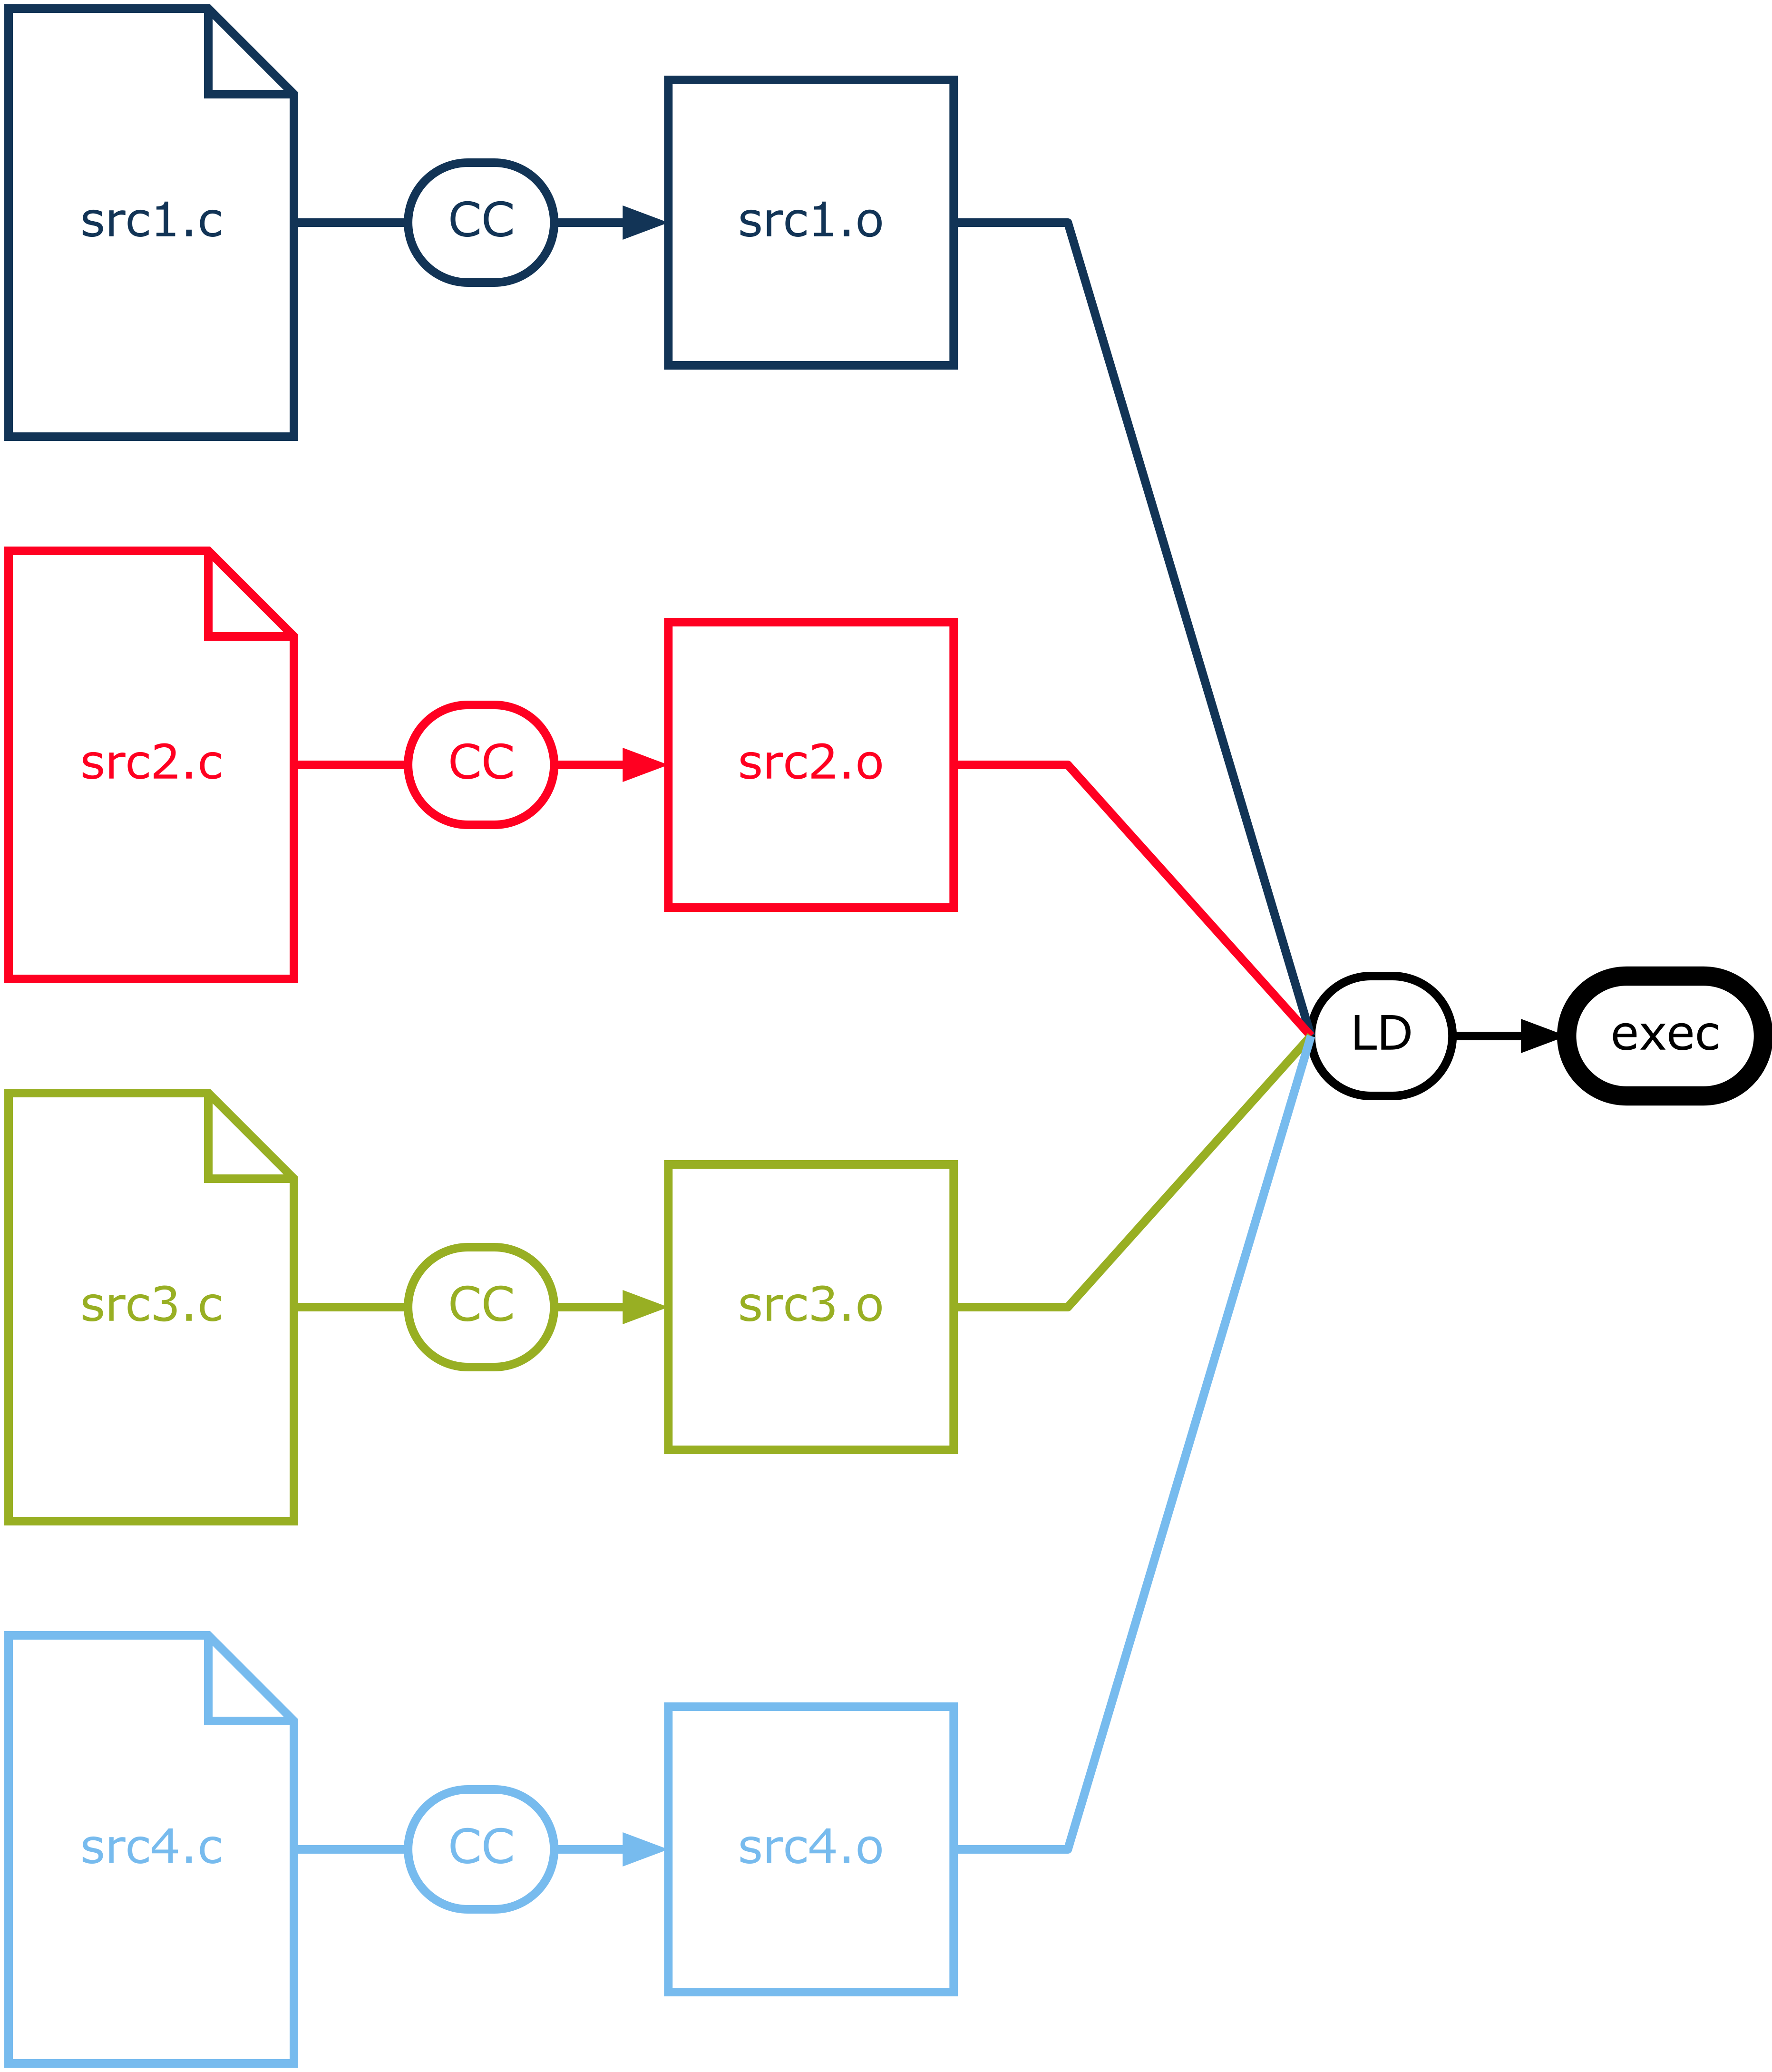
\includegraphics{figures/lb-conf.png}}}
	\caption{A példa projekt vizuális ábrázolása}
	\label{fig:lb-demo-graphic}
\end{figure}

\subsection{Eredmények}\label{sub:results}

Annak érdekében, hogy látható legyen, hogy ezzel a rövid kódrészlettel is lehetséges, jól párhuzamosított kódot megvalósítani, a megvalósított fordító rendszer sebessége egy szintetikus projekt fordításával került lemérésre.
A méréshez használt ,,projekt'' egyes fájljait egy Perl szkript használatával lehetséges legenerálni, amelyik a projekt C++ forrásai mellé egy ,,\texttt{Makefile}'', ,,\texttt{ninja.build}'' és egy ,,\texttt{lb.build}'' fájlt is generál.
Ezekben a fájlokban az egyes források fordításai vannak az adott eszköz szintaktikájával leírva: minden fájl saját szabállyal, mert egyedül a make támogat olyan általános szabályformákat, amelyeket egyszer elég definiálni, és egy makró értékében lévő összes fájlra lehet értelmezni.
A generált C++ forrásfájlok sablon meta--programozással számolják ki a Fibonacci számokat, mindegyik fájl a nevében megadott sorszámút, ezzel elérve azt, hogy nem teljesen triviális az egyes fájlok fordítása, és ezáltal nem az operációs rendszer folyamatindítási idejét mérjük.
A fordítás során kiszámolt értékek a 2000 és 3000 közötti sorszámúak.

A mérésre egy 16 magos (32 hyper-threadinggel) AMD Ryzen 9 7950X processzorral, 64 GiB operatív tárral rendelkező asztali gép volt felhasználva; a diszk, amelyen a mérés történt egy Samsung 990PRO 2 TiB SSD.
A teljes mérés Windows 10 ($10.0.19045.4291$) operációs rendszer alatt történt, a felhasznált MPI megvalósítás MSMPI ($10.1.12498.18$).

A mérés eredményei \aref{fig:bs-speed}.~ábrán és \aref{tbl:bs-speed}.~táblázatban\label{hf:tbl-ref} láthatóak.
Fontos megjegyezni, hogy a Linda megvalósítás esetén az $1$ szálú futtatás eredményekhez hozzátartozik, hogy a rendszer nem támogatja a tisztán soros végrehajtást, így látszólag ,,jobban'' teljesít ebben az esetben, pedig csak az történik, hogy egy--egy fordító és linkelő folyamat indul, ezek viszont képesek parallel is futni, így valamilyen alacsony mértékeben párhuzamosítást valósítanak meg, ami a sok linkelési feladat miatt jelentős sebességnövekedést okoz a mérés során.

\begin{figure}[htb]
	\resizebox{\linewidth}{!}{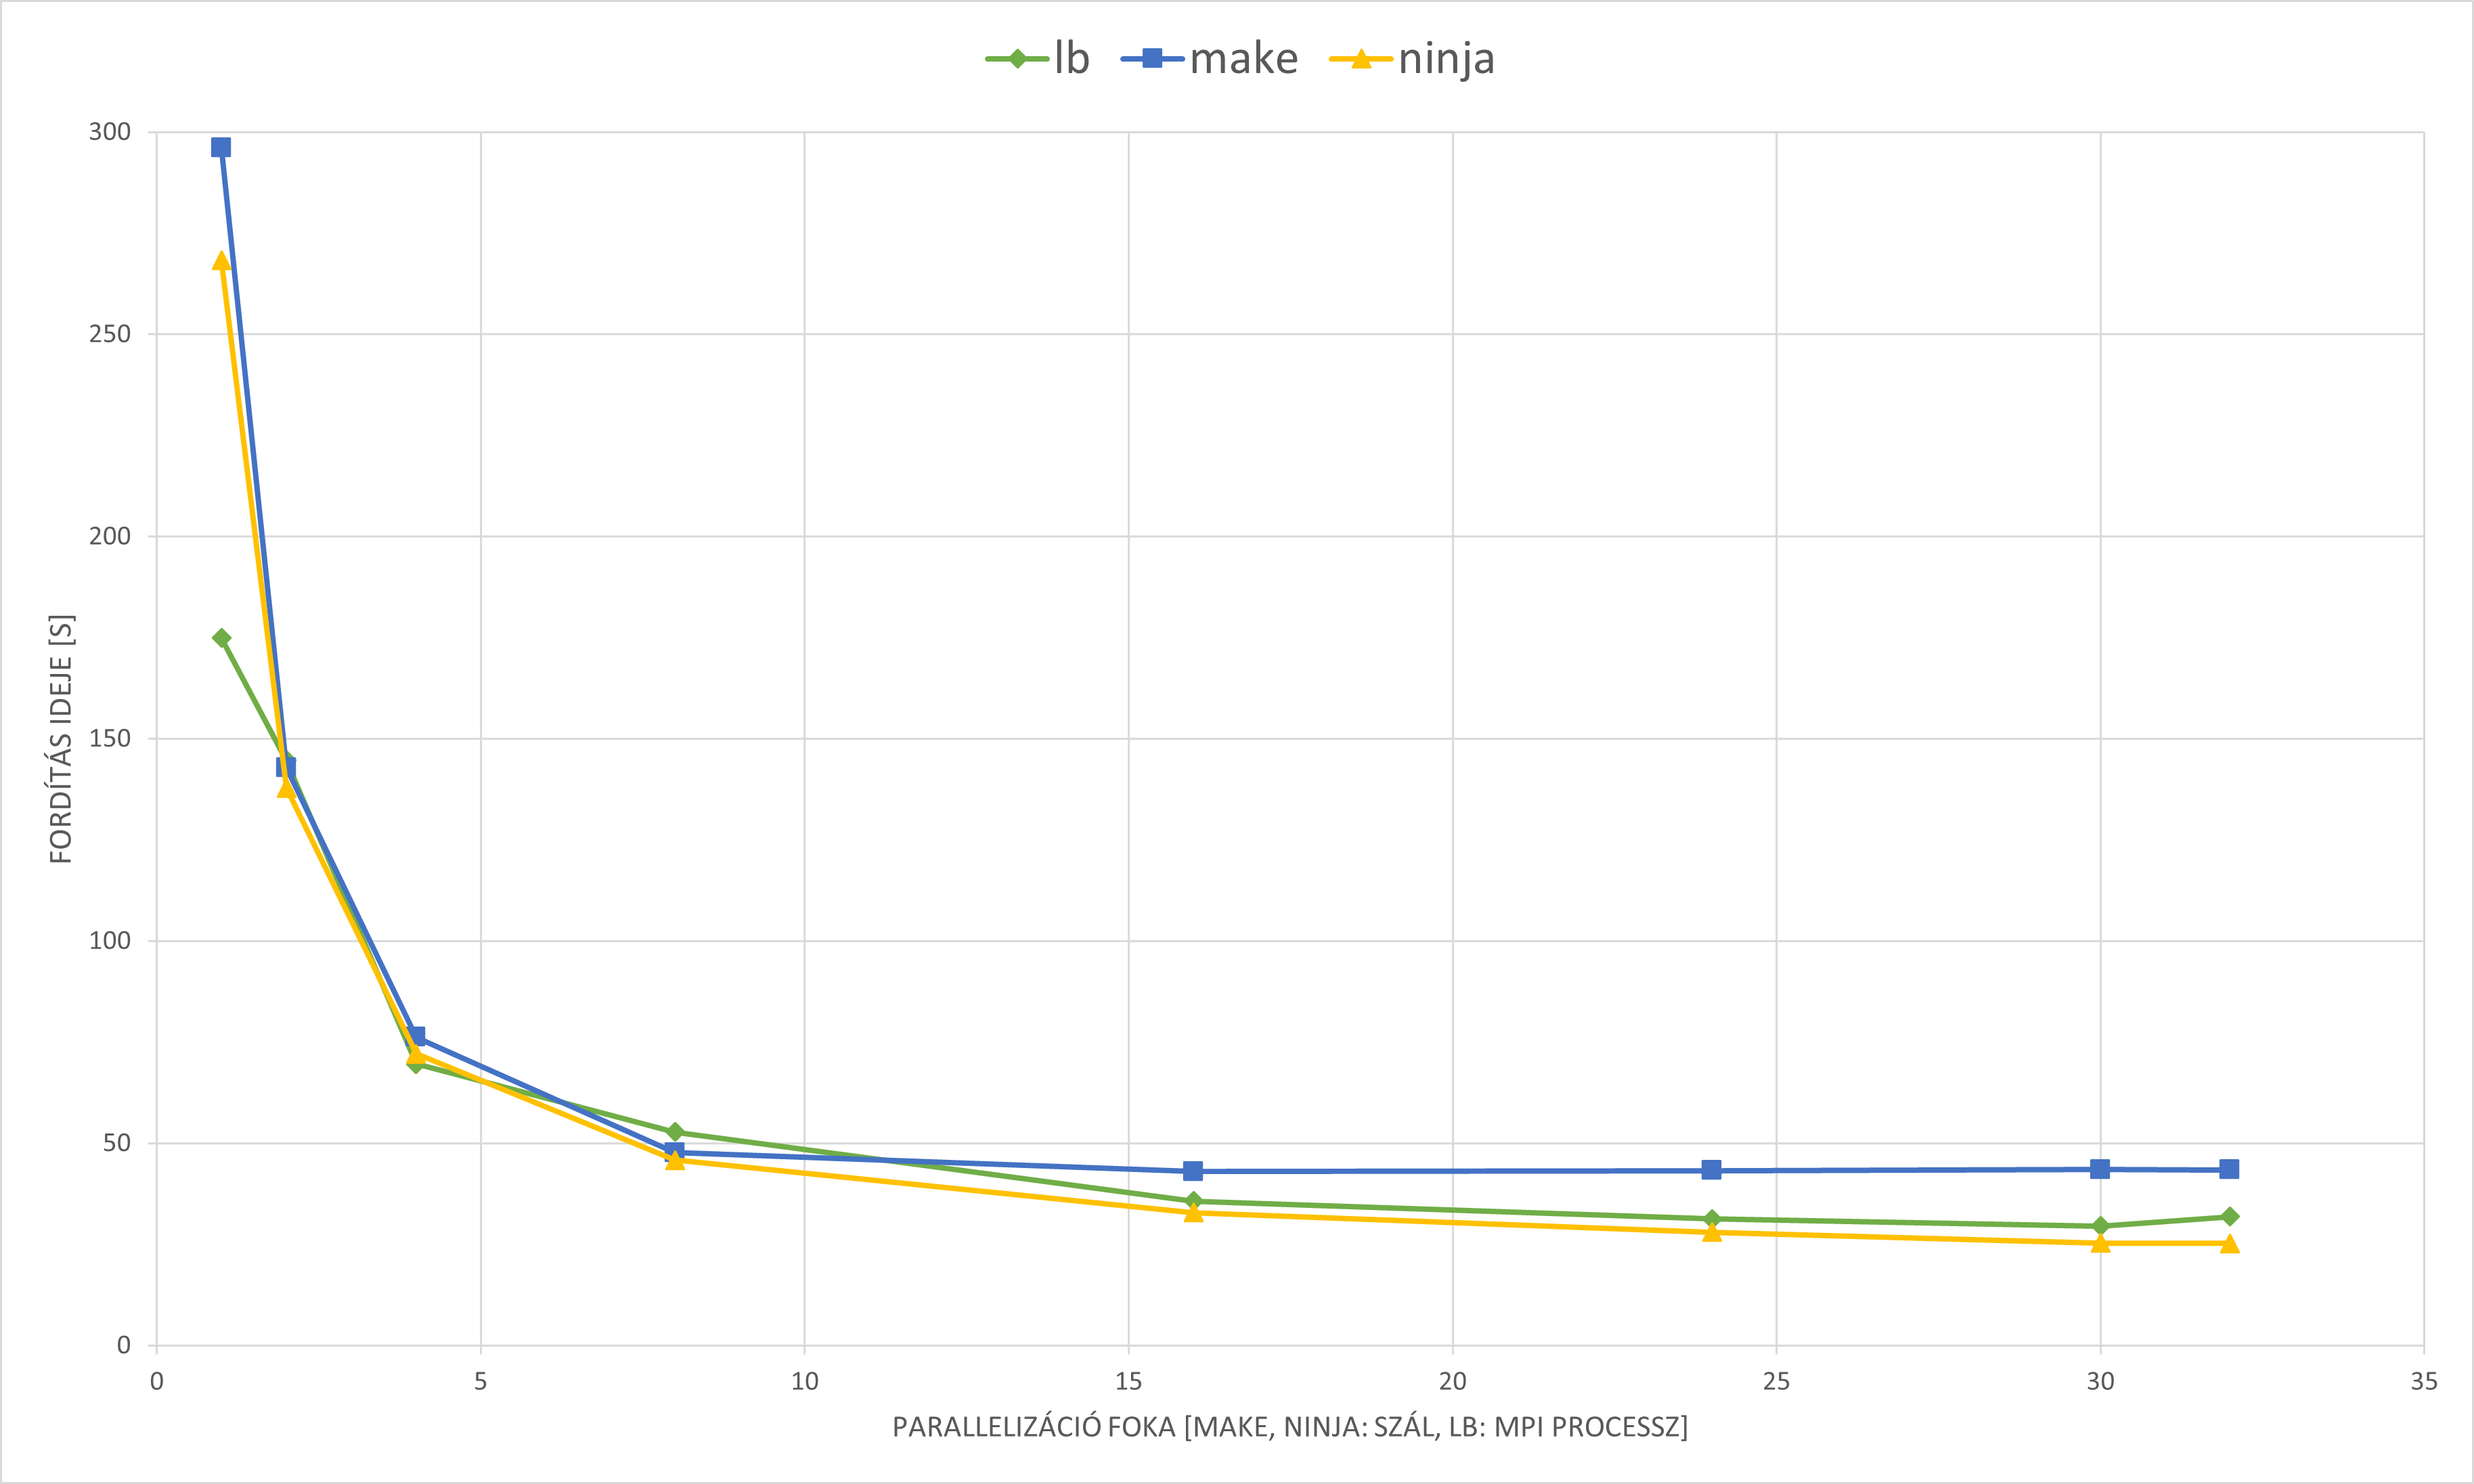
\includegraphics{figures/lb-bench.png}}
	\caption{A különböző rendszerek fordítási sebességei}
	\label{fig:bs-speed}
\end{figure}
	
\begin{table}[htb]
	\begin{tabularx}{\linewidth}{|X||c|c|c|c|c|c|c|c|}
		\hline
		eszköz & 1 & 2 & 4 & 8 & 16 & 24 & 30 & 32 \\
		\hline
		\hline
		make & 296.08 & 142.89 & 76.22 & 47.71 & 43.03 & 43.27 & 43.52 & 43.42 \\
		\hline
		
		ninja & 268.30 & 137.86 & 72.07 & 45.82 & 32.89 & 28.00 & 25.30 & 25.25 \\
		\hline
		
		lb & 174.92 & 144.64 & 69.58 & 52.80 & 35.71 & 31.29 & 29.56 & 31.89 \\
		\hline
	\end{tabularx}
	\caption{A különböző rendszerek fordítási sebességei}
	\label{tbl:bs-speed}
\end{table}



